\section{Svartkroppsstrålning}
\label{sec:blackbody}

Alla objekt reflekterar, absorberar och transmitterar ljus. De kroppar som varken 
reflekterar eller transmitterar något ljus utan absorberar $\unit[100]{\%}$ kallas konventionellt för 
svartkroppar. Detta är en teorektisk konstruktion då perfekta svartkroppar inte existerar 
men trots detta kan en sådan användas som en god modell i flera fysikaliska 
tillämpningar. Den energi som absorberats strålas ut i form av svartkroppsstråling vars 
frekvensspektum bestäms av kroppens temperatur när kroppen är i termisk jämvikt med
 sin omgivning. Den totala utstrålade energin per tidsenhet fås ur Stefan-Boltzmanns lag
 
\begin{equation}
\label{eq:boltzmanslag}
\boxed{ \; \; \;
j^{\star} = \sigma T^{4}
\; \; \; }
\end{equation}

\noindent
där $\sigma$ är Stefan-Boltzmanns konstant som mäts i $\unit{W~m^{-2}~K^{-4}}$ och $T$ är kroppens temperatur vid termisk jämvikt.

\subsection{Härledning}
% av stefan-boltzmanns lag
% med hål i en låda
% kolla i termoboken
I en låda med fotoner kan den totala energin inne i lådan beskrivas som 
\begin{equation}
\label{eq:photonbox}
\frac{U}{V}=\frac{8\pi^5}{15}\frac{(kT)^4}{(hc)^3}
\end{equation}

vilket fås ur Plancks spektrum.\cite[ss.~301-302]{schroeder00}

Sedan görs ett litet hål i lådan, så att några av fotonerna kan slippa ut. Sannolikhet att fotoner med kort respektive lång våglängd ska slippa ut är samma som fördelningen mellan dem inne i lådan, eftersom de har samma hastighet.

\begin{figure}[hpbt]
\centering
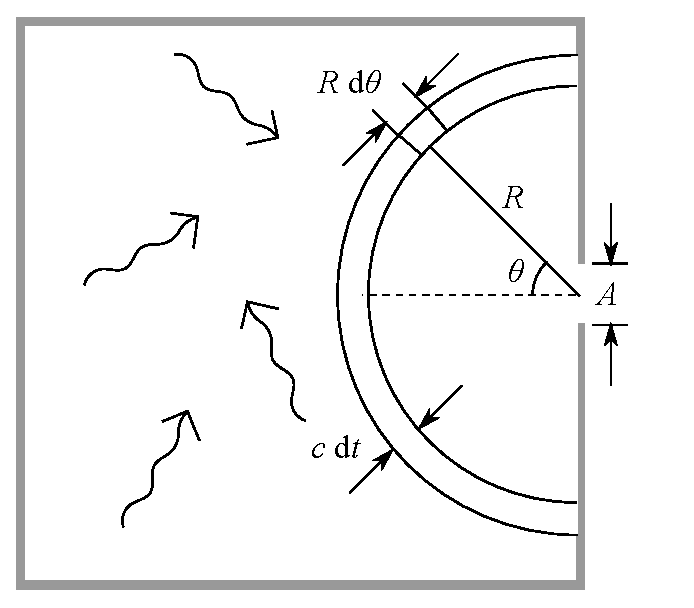
\includegraphics[height=5cm]{images/blackbody_box.eps}
\caption{\label{fig:box}{Fotonerna som lämnar lådan har en liten stund tidigare befunnit sig i samma hemisfär inne i lådan.}}
\end{figure}

Den totala mängden strålning som kommer ut kan då beräknas genom att tänka sig att 
de fotoner som når fram till hålet under en kort tidsperiod, $\mathrm{d}t$, alla befann sig
 i samma hemisfär inne i lådan för en liten stund sedan, se figur \ref{fig:box}. Tjockleken 
 på den tänkta hemisfären är $c\mathrm{d}t$. Hemisfärens radie, $R$, beror givetvis på 
 hur långt bak i tiden vi tittar.

Ett volymelement av hemsfären ges av
\begin{equation}
V=(R\mathrm{d}\theta) \times (R\sin\theta\mathrm{d}\phi) \times (c \mathrm{d}t).
\end{equation}

Energitäthetenför fotonerna i volymelementet är således
\begin{equation}
E_\text{v.e.}=\frac{U}{V} c \mathrm{d}t R^2 \sin\theta \mathrm{d}\theta \mathrm{d}\phi.
\end{equation}

Men endast den andel av fotonerna som har rätt riktning kommer ut genom lådans öppning. Sannoliketen för att en foton har rätt riktning är
\begin{equation}
P(\text{rätt riktning})=\frac{A\cos\theta}{4\pi R^2}
\end{equation}

där A är hålets area. Den totala energin som strålar ut ur hålet från det lilla 
volymselementet är alltså 
\begin{equation}
\frac{A\cos\theta}{4\pi}\frac{U}{V} c\mathrm{d}t \sin\theta\mathrm{d}\theta \mathrm{d}\phi
\end{equation}

vilket ger en total energiutstrålning på
\begin{equation}
\frac{A}{4}\frac{U}{V}c \mathrm{d}t.
\end{equation}

Givetvis är utstrålningen beroende av både hålets area och tidsintervallet. Dividerar vi med dessa storheter får vi effekt per ytenhet, $j$,
\begin{equation}
j=\frac{c}{4}\frac{U}{V}. 
\end{equation}

Sätt in detta uttryck i ekvation~\eqref{eq:photonbox} och ut fås det vi känner som Boltzmans lag,~\eqref{eq:boltzmanslag}
\begin{equation}
j=\frac{2\pi^5}{15}{(kT)^4}{h^3c^2}=\sigma T^4
\end{equation}

där $\sigma=\frac{2\pi^5k^4}{15h^3c^2}$ är Boltzmans konstant.


\subsection{Strålning från omgivningen}
\label{sec:bb_sur}

\begin{figure}[hpbt]
\centering
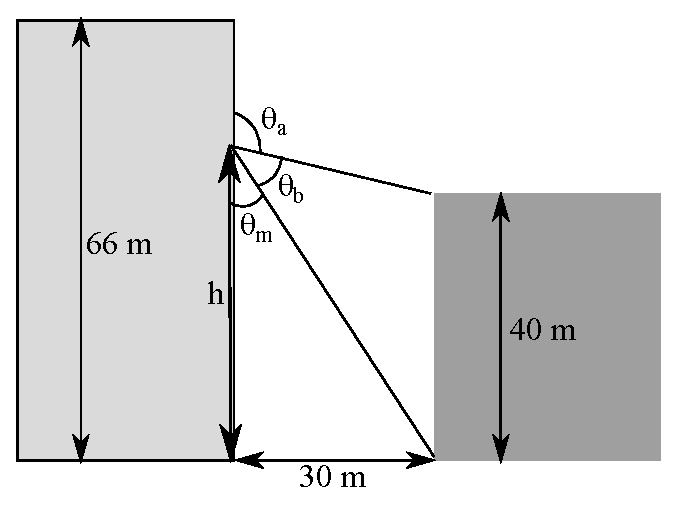
\includegraphics[height=4cm]{images/blackbody_surroundings.eps}
\caption{\label{fig:surroundings}{Så stor andel av den mot väggen instrålande 
svartkroppsstrålningen kommer från olika omgivningar. Den undersökta fastigheten på 
Walleriusgatan t.v., och Johannebergskyrkans församlingshem t.h.}}
\end{figure}

För att uppskatta hur mycket svartkroppsstrålning som kommer mot väggen från olika 
delar av omgivningen sattes en enkel modell upp. Där antas att Johannebergskyrkans 
församlingshem ligger mitt emot vår undersökta fastighet på Walleriusgatan, att 
församlingshemmet ligger 30 meter bort och är 40 meter högt samt att det är det enda 
föremålet av betydande storlek i närheten, se figur~\ref{fig:surroundings}. För varje punkt
 på väggen beskrivs sedan hur stor andel av dess omgivning som upptas av marken, 
 församlingshemmet respektive himlen, eller atmosfären med hjälp av ekvationerna

\begin{equation}
p_\text{gata}=\tan^{-1}(30/h)/180
\end{equation}

\begin{equation}
p_\text{byggnad}= \left\{
\begin{array}{rl}
\tan^{-1}(\frac{30}{h-40})/180 & \text{om } h > 40 \\
(\tan^{-1}(\frac{40-h}{30})+\tan^{-1}(\frac{h}{30}))/180 & \text{om } h < 40 \\
\end{array} \right.
\end{equation}

\begin{equation}
p_\text{atmosfär}=1-p_\text{gata}-p_\text{byggnad}.
\end{equation}

Medelvärdet då h går från 0 till 66 meter ger det genomsnittliga värdet för hur stor andel 
av den instrålade svartkroppsstrålningen mot hela väggen som kommer från olika delar
 av omgivningen. Detta ger resultatet att 26\% kommer från gata, 36\% från 
 församlingshemmet och 38\% från atmosfären. Oftast antas allt som inte är atmosfären att ha utomhustemperatur.
 
Atmosfärens temperatur kan fås ur \cite{bb_atmosphere}, där Stephan-Boltzmans lag modifieras och att strålningen från atmosfären en klar dag kan beskrivas som 
\begin{equation}
I_\text{atmosfär}=\sigma\cdot T_\text{ute}^4(1-c \cdot e^{-d(273-T_\text{ute})^2})
\end{equation}
där $c=0,261$ och $d=7,77\cdot10^{-4}$ kommer ur statistiska data. En helt molnig dag kan atmosfärens temperatur $T_\text{ute}$, det vill säga $c=0$. Denna ekvation har fåtts ut statistiska data från flera olika platser över hela världen. 